%% chapter13_slides.tex  -  Chapter 13: A Bayesian Investment Analyst on the
%% Johannesburg Stock Exchange
%% Bayesian Machine Learning in Quantitative Finance: Theory and Practical
%% Applications -- Mongwe, Mbuvha & Marwala (Springer, 2025)
%% Compile: pdflatex -interaction=nonstopmode chapter13_slides.tex  (twice)
\documentclass[aspectratio=169,10pt]{beamer}

\usetheme{Madrid}
\usecolortheme{seahorse}
\usefonttheme{professionalfonts}

%% packages
\usepackage{amsmath,amssymb,mathtools}
\usepackage{mathrsfs}
\usepackage{bm}
\usepackage{graphicx}
\usepackage{booktabs}
\usepackage{array}
\usepackage{listings}
\usepackage{xcolor}
\usepackage{tikz}

\graphicspath{{figures/}}

%% listings style
\definecolor{codegray}{rgb}{0.95,0.95,0.95}
\lstdefinestyle{pycode}{
  language=Python,
  basicstyle=\ttfamily\scriptsize,
  keywordstyle=\color{blue!60!black}\bfseries,
  commentstyle=\color{green!50!black}\itshape,
  stringstyle=\color{orange!80!black},
  numbers=left,
  numberstyle=\tiny\color{gray},
  numbersep=5pt,
  frame=single,
  backgroundcolor=\color{gray!7},
  tabsize=2,
  showstringspaces=false,
  breaklines=true,
  captionpos=b,
}
\lstset{style=pycode}

%% footline / navigation
\setbeamertemplate{footline}[frame number]
\setbeamertemplate{navigation symbols}{}

%% macros
\newcommand{\R}{\mathbb{R}}
\newcommand{\Prob}{\mathbb{P}}
\renewcommand{\Pr}{\mathbb{P}}
\newcommand{\Ex}{\mathbb{E}}
\newcommand{\w}{\mathbf{w}}
\newcommand{\x}{\mathbf{x}}
\newcommand{\y}{\mathbf{y}}
\newcommand{\p}{\mathbf{p}}
\newcommand{\M}{\mathbf{M}}
\newcommand{\Data}{\mathrm{D}}
\newcommand{\sig}{\sigma}

%%=============================================================================
\title[Bayesian ML in QF -- Ch.13]{Bayesian Machine Learning in Quantitative Finance}
\subtitle{Chapter 13: A Bayesian Investment Analyst on the JSE}
\author{Based on Mongwe, Mbuvha \& Marwala}
\date{}

%%=============================================================================
\begin{document}

\begin{frame}
  \titlepage
\end{frame}

\begin{frame}{Chapter Outline}
  \tableofcontents
\end{frame}

%%=============================================================================
\section{Notation \& Recap}
%%=============================================================================

\begin{frame}[allowframebreaks]{Notation You'll Need / Recap}

This chapter is an \emph{application} chapter: it takes the Bayesian logistic
regression model (Ch.~2/6) and the MALA / HMC / S2HMC samplers (Ch.~3, 7, 9,
11) that you already know in detail, and uses all three \emph{together, on
the same model and the same data}, to build and compare a "Bayesian
investment analyst" that reads sell-side analyst reports on JSE-listed stocks
and predicts whether the report's price call will turn out to be directionally
correct.

\begin{block}{Recap: Bayesian Logistic Regression (Ch.~2/6)}
For a binary label $y\in\{0,1\}$ and feature vector $\x\in\R^d$, the
likelihood is Bernoulli with success probability $\sig(\w^\top\x)$, where
$\sig(z)=1/(1+e^{-z})$ is the logistic sigmoid. Placing a prior on $\w$ and
combining with the likelihood via Bayes' theorem gives a posterior
$p(\w\mid \Data)$ that has \emph{no closed form} once you multiply a
non-Gaussian likelihood by even a Gaussian prior --- hence the need for MCMC.
\end{block}

\begin{block}{Recap: MALA / HMC / S2HMC (Ch.~3, 7, 9, 11)}
All three are \emph{gradient-informed} MCMC methods that use $\nabla_\w \ln
p(\w\mid\Data)$ to propose better-than-random-walk moves:
\begin{itemize}
  \item \textbf{MALA} -- one step of discretised Langevin diffusion (drift =
        gradient, diffusion = Brownian noise) + a Metropolis correction.
  \item \textbf{HMC} -- simulates Hamiltonian dynamics with a leapfrog
        integrator over $L$ steps, then Metropolis-corrects for the
        discretisation error; MALA is the special case $L=1$.
  \item \textbf{S2HMC} -- runs leapfrog on a \emph{shadow} (modified)
        Hamiltonian that the integrator conserves more accurately, raising
        the acceptance rate and reducing autocorrelation relative to HMC.
\end{itemize}
\end{block}

\framebreak

\begin{alertblock}{What's New in This Chapter: Two Things}
\begin{enumerate}
  \item \textbf{The features are analyst-report-derived, not asset returns.}
        Each "data point" is one sell-side report on one JSE stock, described
        by features like its target price, rating, volatility context, and
        past accuracy record (Sect.~13.4.1) --- not a raw price series. The
        label is \emph{bidirectional accuracy}: did the stock actually move
        in the direction the report implied?
  \item \textbf{MALA, HMC and S2HMC are run side by side and compared}, not
        just used once to fit a model. The chapter trains the \emph{same}
        Bayesian logistic regression model three times (once per sampler) on
        four datasets (full JSE universe + 3 sectors) and compares them on
        (a) predictive AUC, (b) effective sample size (ESS) and ESS
        normalised by execution time, and (c) which features each sampler's
        posterior ranks as most important.
\end{enumerate}
\end{alertblock}

\begin{block}{How Report Features Feed the Model}
Every sell-side report is converted into a numeric feature vector $\x_i$
(target price, rating, volatility measures, past-accuracy scores, \ldots --
14 features in total, Sect.~13.4.1). The model then places an
\textbf{automatic relevance determination (ARD) prior} over the logistic
regression weight vector $\w$, so that after training, the \emph{posterior
variance} of each weight automatically tells you how important the
corresponding report feature was for predicting bidirectional accuracy --
this is what makes the model "explainable" to an analyst, not just
predictive.
\end{block}

\end{frame}

%%=============================================================================
\section{13.1 Introduction}
%%=============================================================================

\begin{frame}[allowframebreaks]{13.1 \; Introduction: Why Model Sell-Side Analyst Reports?}

\begin{block}{The Business Problem}
Sell-side analysts publish reports with a \textbf{target price}, an
\textbf{earnings forecast}, and a \textbf{rating} (Strong Sell / Sell / Hold
/ Buy / Strong Buy). Institutional investors (pension funds, asset managers)
use these reports for portfolio decisions, so the \emph{accuracy} of the
reports matters a great deal.
\begin{itemize}
  \item \textbf{Point accuracy}: how close is the target price to the actual
        realised price?
  \item \textbf{Directional (bidirectional) accuracy}: did the stock move in
        the \emph{direction} the report implied? Many traders act on
        direction, not on the exact target level --- this is the chapter's
        focus.
\end{itemize}
\end{block}

\begin{alertblock}{Known Issues with Analyst Reports}
\begin{itemize}
  \item Conflicts of interest: analysts may align forecasts with their own
        economic incentives, or herd toward a consensus with other analysts.
  \item Coverage is skewed toward blue-chip stocks, with mid-/small-caps
        under-covered.
  \end{itemize}
These issues motivate combining \emph{many} analysts' reports with a
data-driven model rather than trusting any single report.
\end{alertblock}

\framebreak

\begin{block}{From "AI Analyst" to "Bayesian Analyst"}
Sidogi et al. (2022) proposed an \textbf{"AI analyst"}: use random forests
and deep neural networks to fuse sell-side report features into directional
forecasts for FTSE/JSE All Share Index companies, with little human
involvement. \textbf{This chapter extends that idea into the Bayesian
framework}: the same directional-forecast task, but with
\begin{itemize}
  \item a \textbf{Bayesian logistic regression with ARD prior} (BLR-ARD)
        instead of a black-box ensemble/deep net, and
  \item \textbf{MCMC} (MALA, HMC, S2HMC) instead of point-estimate training,
        so that predictions come with \emph{quantified uncertainty} and
        features come with an automatically learned \emph{importance
        ranking}.
\end{itemize}
\end{block}

\begin{block}{Why Bayesian?}
The Bayesian framework answers two questions the frequentist "AI analyst"
cannot answer directly:
\begin{enumerate}
  \item \textbf{How confident is the model?} -- the posterior over $\w$
        gives a full predictive distribution, not just a point probability.
  \item \textbf{Which features actually matter?} -- the ARD prior's
        per-feature variance hyperparameters $\alpha_i$ give a principled,
        automatically-learned feature-importance ranking (no separate
        feature-selection step needed).
\end{enumerate}
\end{block}

\begin{block}{Headline Finding (previewed)}
The BLR-ARD model \textbf{outperforms on industrial and resource-sector
stocks}, with \textbf{financial stocks} showing the lowest bidirectional
accuracy. \textbf{Volatility-related features, plus the initial and target
price}, are consistently important drivers of directional predictability
across sectors (details in Sect.~13.5).
\end{block}

\end{frame}

%%=============================================================================
\section{13.2 Bayesian Logistic Regression Model}
%%=============================================================================

\begin{frame}{13.2 \; Setting Up the Model: Intuition}
  \begin{columns}
    \column{0.55\textwidth}
      \begin{block}{Intuition}
        We want $\Pr(\text{stock moves as the report implied} \mid
        \text{report features})$. Logistic regression is the natural choice:
        it maps a linear combination of report features through a sigmoid to
        get a probability in $[0,1]$. Being \emph{Bayesian} about $\w$ means
        we don't just get one "best" probability -- we get a whole
        \emph{distribution} over plausible probabilities, reflecting how much
        the (finite, noisy) report history really tells us.
      \end{block}
    \column{0.42\textwidth}
      \centering
      {\small Report features $\x_i$ (target price, rating, volatility, \ldots)
      $\;\longrightarrow\;$ linear score $\w^\top\x_i$ $\;\longrightarrow\;$
      sigmoid $\;\longrightarrow\;$ $\Pr(y_i{=}1)$}
  \end{columns}
\end{frame}

\begin{frame}{13.2 \; The Likelihood (Eq.~13.1)}
  \begin{block}{Negative Log-Likelihood}
    \[
      l(\Data\mid\w) = \sum_{i}^{N} y_i\log(\w^\top x_i) + (1-y_i)\log(1-\w^\top x_i)
    \]
    \begin{tabular}{ll}
      $\Data=\{\x,y\}$ & the data: report feature vectors $\x$ and bidirectional-accuracy labels $y$\\
      $N$              & number of observations (analyst reports)\\
      $\w$              & the parameters (weights) to be estimated\\
    \end{tabular}
  \end{block}
  \vspace{4pt}
  As printed in the book (Marwala et al., 2023; Mongwe et al., 2021c), the
  term $\w^\top x_i$ here plays the role of the predicted probability
  $p_i=\sig(\w^\top x_i)$ under the usual logistic link -- i.e.\ this is the
  standard Bernoulli cross-entropy log-likelihood
  $\sum_i y_i\log p_i + (1-y_i)\log(1-p_i)$ with $p_i=\sig(\w^\top x_i)$; we
  use this explicit sigmoid form on the next slide to derive the gradient.
\end{frame}

\begin{frame}{13.2 \; The Posterior and the ARD Prior (Eq.~13.2)}
  \begin{block}{Un-normalised Log Posterior}
    \[
      \ln p(\w\mid \Data) = l(\Data\mid\w) + \ln p(\w\mid\alpha) + \ln q(\alpha)
    \]
    \begin{tabular}{ll}
      $\ln p(\w\mid\alpha)$ & log prior on weights given hyperparameters $\alpha$\\
      $\ln q(\alpha)$        & log distribution of the hyperparameters $\alpha$\\
    \end{tabular}
  \end{block}
  \begin{alertblock}{Automatic Relevance Determination (ARD)}
    Each weight $w_j$ has its \textbf{own} Gaussian prior, zero mean, variance
    $\alpha_j$: $w_j\mid\alpha_j\sim\mathcal N(0,\alpha_j)$, with
    $\alpha_j\sim\text{LogNormal}(0,1)$.
    \begin{itemize}
      \item \textbf{Large $\alpha_j$} $\Rightarrow$ $w_j$ can be large
            $\Rightarrow$ feature $j$ is \emph{important}.
      \item \textbf{Small $\alpha_j$} $\Rightarrow$ $w_j$ is shrunk toward
            $0$ $\Rightarrow$ feature $j$ is \emph{irrelevant}.
    \end{itemize}
    Both $\w$ and $\alpha$ are \textbf{jointly sampled} by MCMC in this
    chapter (doubling the parameter space vs. Gibbs-sampling $\alpha$
    separately, but giving more stable exploration, Mongwe et al., 2021c).
  \end{alertblock}
\end{frame}

\begin{frame}[allowframebreaks]{13.2 \; Deriving the Gradient, Step by Step (Toy 2-Feature Case)}

\begin{alertblock}{Why We Need This}
Both MALA (Eq.~13.3) and HMC (Eq.~13.4) need $\nabla_\w \ln p(\w\mid\Data)$.
We derive it here explicitly for a toy case with just \textbf{two features}
$x_{i1},x_{i2}$ (e.g.\ "sentiment score" and "EPS revision"), so $\w=(w_1,w_2)$
and $p_i=\sig(w_1 x_{i1}+w_2 x_{i2})$.
\end{alertblock}

\begin{block}{Step 1: Write the Log-Likelihood in Sigmoid Form}
\[
  l(\Data\mid\w) = \sum_{i=1}^N \Big[y_i\log p_i + (1-y_i)\log(1-p_i)\Big], \qquad p_i=\sig(w_1x_{i1}+w_2x_{i2})
\]
\end{block}

\begin{block}{Step 2: Differentiate the Sigmoid}
Using the standard identity $\dfrac{d\sig(z)}{dz}=\sig(z)(1-\sig(z))$ and the
chain rule, for $j=1,2$:
\[
  \frac{\partial p_i}{\partial w_j} = p_i(1-p_i)\,x_{ij}
\]
\end{block}

\framebreak

\begin{block}{Step 3: Differentiate Each Term of the Log-Likelihood}
\[
  \frac{\partial}{\partial w_j}\big[y_i\log p_i\big]
  = \frac{y_i}{p_i}\cdot p_i(1-p_i)x_{ij} = y_i(1-p_i)x_{ij}
\]
\[
  \frac{\partial}{\partial w_j}\big[(1-y_i)\log(1-p_i)\big]
  = \frac{-(1-y_i)}{1-p_i}\cdot p_i(1-p_i)x_{ij} = -(1-y_i)p_i\,x_{ij}
\]
\end{block}

\begin{block}{Step 4: Add the Two Pieces --- They Telescope}
\[
  y_i(1-p_i)x_{ij} - (1-y_i)p_i\,x_{ij}
  = \big[y_i - y_ip_i - p_i + y_ip_i\big]x_{ij} = (y_i-p_i)\,x_{ij}
\]
So the gradient of the log-likelihood, summed over reports, is remarkably
simple:
\[
  \boxed{\frac{\partial l(\Data\mid\w)}{\partial w_j} = \sum_{i=1}^N (y_i-p_i)\,x_{ij}}
\]
\end{block}

\framebreak

\begin{block}{Step 5: Add the Gradient of the ARD Log-Prior}
$\ln p(\w\mid\alpha) = -\tfrac12\sum_j w_j^2/\alpha_j + \text{const}$, so
\[
  \frac{\partial \ln p(\w\mid\alpha)}{\partial w_j} = -\frac{w_j}{\alpha_j}
\]
\end{block}

\begin{block}{Step 6: The Full Gradient, for Our Toy 2-Feature Case}
\[
  \frac{\partial \ln p(\w\mid\Data)}{\partial w_1}
    = \sum_{i=1}^N (y_i-p_i)\,x_{i1} - \frac{w_1}{\alpha_1}, \qquad
  \frac{\partial \ln p(\w\mid\Data)}{\partial w_2}
    = \sum_{i=1}^N (y_i-p_i)\,x_{i2} - \frac{w_2}{\alpha_2}
\]
In vector form, this is exactly $f'(\w)$ in MALA's Eq.~13.3 and
$-\partial H(\w,\p)/\partial\w$ in HMC's Eq.~13.4:
\[
  \nabla_\w \ln p(\w\mid\Data) = \x^\top(\y-\p_{\text{prob}}) - \w\oslash\bm\alpha
\]
where $\oslash$ is element-wise division and $\p_{\text{prob}}=(p_1,\ldots,p_N)$
stacks the predicted probabilities. This same formula, extended from $2$ to
$14$ features, is what all three samplers use in the real JSE experiments.
\end{block}

\end{frame}

\begin{frame}{13.2 \; Toy Running Example: 5 Fictional Analyst Reports}
  \begin{block}{Intuition}
    To make the model concrete, we build a tiny toy "sell-side report"
    dataset by hand: 5 fictional reports, each with a conviction-strength
    feature vector, and a binary label for whether the call was
    bidirectionally correct. This is \textbf{entirely fictional} -- a
    pedagogical stand-in for the book's real 29{,}935-report Bloomberg
    dataset (Sect.~13.4.1).
  \end{block}
  \begin{center}
  \begin{tabular}{lccccc}
    \toprule
    Report (fictional) & Rating & $|$sentiment$|$ & $|$EPS rev.$|$ & $|$target-price chg.$|$ & $y$ (correct?)\\
    \midrule
    Alpha Capital     & Buy  & 0.80 & 0.060 & 0.120 & 1\\
    Beta Securities   & Sell & 0.60 & 0.040 & 0.080 & 1\\
    Gamma Research    & Hold & 0.10 & 0.005 & 0.010 & 0\\
    Delta Equities    & Buy  & 0.50 & 0.030 & 0.070 & 1\\
    Epsilon Analytics & Hold & 0.20 & 0.005 & 0.015 & 0\\
    \bottomrule
  \end{tabular}
  \end{center}
  \vspace{6pt}
  \textbf{Toy story:} reports with \emph{stronger conviction} (larger-magnitude
  signals, either bullish or bearish) tend to be vindicated more often than
  wishy-washy "Hold" calls with near-zero conviction -- so all three features
  are conviction \emph{magnitudes}, and the ARD prior gets to decide how much
  each one matters.
\end{frame}

\begin{frame}[fragile]{Python: BLR-ARD Log Posterior and Gradient}
\begin{lstlisting}[caption={From-scratch log posterior and analytic gradient (Eqs. 13.1-13.2, and the derivation above)}]
import numpy as np

# Toy dataset: 5 fictional analyst reports (bias + 3 features)
X_raw = np.array([[0.80, 0.060, 0.120],   # Alpha Capital  (Buy)
                   [0.60, 0.040, 0.080],   # Beta Securities (Sell)
                   [0.10, 0.005, 0.010],   # Gamma Research (Hold)
                   [0.50, 0.030, 0.070],   # Delta Equities (Buy)
                   [0.20, 0.005, 0.015]])  # Epsilon Analytics (Hold)
y = np.array([1, 1, 0, 1, 0])
X = np.hstack([np.ones((5, 1)), X_raw])       # prepend bias column
alpha = np.array([4.0, 4.0, 4.0, 4.0])        # fixed ARD prior variances (toy)

def sigmoid(z):
    return 1.0 / (1.0 + np.exp(-z))

def log_posterior(w):
    """ln p(w|D): Bernoulli log-lik (Eq. 13.1) + Gaussian ARD log-prior."""
    p = sigmoid(X @ w)
    ll = np.sum(y * np.log(p) + (1 - y) * np.log(1 - p))
    log_prior = -0.5 * np.sum(w**2 / alpha)
    return ll + log_prior

def grad_log_posterior(w):
    """Analytic gradient derived step-by-step above: sum_i (y_i-p_i)x_i - w/alpha."""
    p = sigmoid(X @ w)
    return X.T @ (y - p) - w / alpha
\end{lstlisting}
\end{frame}

%%=============================================================================
\section{13.3 Markov Chain Monte Carlo Algorithms}
%%=============================================================================

\begin{frame}{13.3 \; Three Samplers, One Posterior}
  \begin{block}{Intuition}
    All three samplers target the \emph{same} un-normalised posterior
    $p(\w\mid\Data)$ from Eq.~13.2 -- they differ only in \emph{how} they
    propose moves through $\w$-space. The chapter's central experiment is not
    "which sampler do we pick?" but \textbf{"how do MALA, HMC, and S2HMC
    compare on the exact same BLR-ARD model and the exact same JSE data?"}
    (Sect.~13.4-13.5).
  \end{block}
  \begin{center}
    \begin{tabular}{lccc}
      \toprule
       & MALA & HMC & S2HMC\\
      \midrule
      Gradient order used     & 1st & 1st & 1st (via shadow Ham.)\\
      Trajectory length $L$   & $1$ (implicit)  & tunable ($15$ in this chapter) & tunable ($15$ in this chapter)\\
      Target accept.\ rate    & $60\%$ & $80\%$ & $80\%$\\
      Relative auto-correlation & highest & lower & lowest\\
      \bottomrule
    \end{tabular}
  \end{center}
\end{frame}

\begin{frame}{13.3.1 \; MALA -- Efficient Recap}
  \begin{block}{Langevin Dynamics (Eq.~13.3)}
    \[
      d\w_t = \tfrac12 f'(\w)\,dt + dZ_t
    \]
    \begin{tabular}{ll}
      $\w$    & the parameters\\
      $f'(\w)$ & first derivative of the target $f(\w)=\ln p(\w\mid\Data)$ w.r.t.\ $\w$\\
      $Z_t$    & Brownian motion at fictitious time $t$\\
    \end{tabular}
  \end{block}
  \begin{itemize}
    \item Discretised via Euler-Maruyama $\Rightarrow$ a Gaussian proposal
          centred at $\w+\tfrac12\epsilon f'(\w)$; a Metropolis correction
          fixes the resulting detailed-balance violation.
    \item Converges faster than plain Metropolis-Hastings because it uses
          first-order gradient information -- but samples are \textbf{still
          highly correlated} (it is, after all, a single-leapfrog-step
          special case of HMC).
  \end{itemize}
  \vspace{4pt}
  \textbf{This chapter's specifics:} step size tuned via dual averaging
  (Hoffman \& Gelman, 2014) to a target acceptance rate of $60\%$.
\end{frame}

\begin{frame}[fragile]{Python: MALA Sampler for the Toy Analyst Model}
\begin{lstlisting}[caption={From-scratch MALA (Eq. 13.3 + Metropolis correction) on the toy BLR-ARD posterior}]
def run_mala(n_iter, step, dim, log_posterior, grad_log_posterior, rng):
    w = np.zeros(dim)
    lp, grad = log_posterior(w), grad_log_posterior(w)
    chain = np.zeros((n_iter, dim))
    for m in range(n_iter):
        mean_fwd = w + 0.5 * step * grad                    # Langevin drift
        prop = mean_fwd + np.sqrt(step) * rng.standard_normal(dim)
        lp_prop = log_posterior(prop)
        grad_prop = grad_log_posterior(prop)
        mean_bwd = prop + 0.5 * step * grad_prop
        # Metropolis correction for the asymmetric Gaussian proposal
        log_q_fwd = -np.sum((prop - mean_fwd)**2) / (2 * step)
        log_q_bwd = -np.sum((w - mean_bwd)**2) / (2 * step)
        log_accept = (lp_prop + log_q_bwd) - (lp + log_q_fwd)
        if np.log(rng.uniform()) < log_accept:
            w, lp, grad = prop, lp_prop, grad_prop           # accept
        chain[m] = w
    return chain
\end{lstlisting}
\end{frame}

\begin{frame}{13.3.2 \; HMC -- Efficient Recap}
  \begin{block}{Hamiltonian Dynamics (Eq.~13.4)}
    \[
      \frac{d\w}{dt} = \frac{\partial H(\w,\p)}{\partial\p}, \qquad
      \frac{d\p}{dt} = -\frac{\partial H(\w,\p)}{\partial\w}
    \]
    \begin{tabular}{ll}
      $\p$      & auxiliary momentum, same dimension as $\w$\\
      $H(\w,\p)$ & Hamiltonian = potential (target posterior) + kinetic (Gaussian) energy\\
    \end{tabular}
  \end{block}
  \begin{block}{Leapfrog + Metropolis Correction (Eqs.~13.5-13.6)}
    Leapfrog integrates the dynamics for $L$ steps of size $\epsilon$; then
    \[
      \Pr(\text{accept } \w^*) = \min\left(1,\ \frac{\exp(-H(\w^*,\p^*))}{\exp(-H(\w,\p))}\right)
    \]
    corrects for the $\mathcal O(\epsilon^2)$ discretisation error. Setting
    $L=1$ recovers MALA exactly.
  \end{block}
  \textbf{This chapter's specifics:} step size $\epsilon$ tuned by dual
  averaging to an $80\%$ target acceptance rate; trajectory length
  \textbf{fixed at $L=15$} for all four experiments.
\end{frame}

\begin{frame}[fragile]{Python: HMC Sampler for the Toy Analyst Model}
\begin{lstlisting}[caption={From-scratch HMC (leapfrog, Eq. 13.5, + acceptance, Eq. 13.6) on the toy posterior}]
def run_hmc(n_iter, eps, L, dim, log_posterior, grad_log_posterior, rng):
    w = np.zeros(dim)
    chain = np.zeros((n_iter, dim))
    for m in range(n_iter):
        p0 = rng.standard_normal(dim)                 # draw momentum
        w_new, p = w.copy(), p0.copy()
        grad = grad_log_posterior(w_new)
        for _ in range(L):                            # leapfrog, Eq. 13.5
            p = p + 0.5 * eps * grad
            w_new = w_new + eps * p
            grad = grad_log_posterior(w_new)
            p = p + 0.5 * eps * grad
        H0 = -log_posterior(w) + 0.5 * np.sum(p0**2)      # potential + kinetic
        H1 = -log_posterior(w_new) + 0.5 * np.sum(p**2)
        if np.log(rng.uniform()) < (H0 - H1):             # Eq. 13.6
            w = w_new
        chain[m] = w
    return chain
\end{lstlisting}
\end{frame}

\begin{frame}[allowframebreaks]{13.3.3 \; S2HMC -- Efficient Recap}

\begin{alertblock}{The Problem HMC Still Has}
Leapfrog only conserves $H$ to $\mathcal O(\epsilon^2)$, so $H$ still drifts
along a trajectory -- causing rejections in the Metropolis step. Fix:
integrate a \textbf{shadow Hamiltonian} $\tilde H$ that leapfrog conserves
far more accurately.
\end{alertblock}

\begin{block}{Shadow Hamiltonian Expansion (Eqs.~13.7-13.9)}
\[
  \tilde H = H + \epsilon H_2 + \epsilon^2 H_3 + \epsilon^3 H_4 + \ldots, \qquad
  \tilde H^{[k]} = \tilde H + \mathcal O(\epsilon^k)
\]
A 4th-order truncation for leapfrog is
\[
  \tilde H^{[4]} = \mathrm U(\w)+\mathrm K(\p) + \frac{\epsilon^2}{12}\mathrm K_\p^\top \mathrm U_{\w\w}\mathrm K_\p - \frac{\epsilon^2}{24}\mathrm U_\w^\top \mathrm K_{\p\p}\mathrm U_\w + \mathcal O(\epsilon^4)
\]
but this is \textbf{non-separable} in $(\w,\p)$ -- expensive to tune.
\end{block}

\framebreak

\begin{block}{Making It Separable: S2HMC (Eq.~13.10)}
Sweet et al.\ (2009) pre-process $(\w,\p)$ through the leapfrog integrator to
get a \textbf{separable} shadow Hamiltonian:
\[
  \tilde H(\w,\p) = \mathrm U(\w)+\mathrm K(\p) + \frac{\epsilon^2}{24}\mathrm U_\w^\top \M^{-1} \mathrm U_\w + \mathcal O(\epsilon^4)
\]
\begin{tabular}{ll}
  $\mathrm U(\w)$ & potential energy $=-\ln p(\w\mid\Data)$\\
  $\mathrm K(\p)$ & kinetic energy $=\tfrac12\p^\top\M^{-1}\p$\\
  $\mathrm U_\w,\mathrm U_{\w\w}$ & Jacobian / Hessian of $\mathrm U$; $\mathrm K_\p,\mathrm K_{\p\p}$ analogous for $\mathrm K$\\
\end{tabular}
\end{block}

\begin{block}{Reversible Pre-/Post-Processing (Eqs.~13.11-13.14)}
Before leapfrog, map $(\w,\p)\mapsto(\hat\w,\hat\p)$ by fixed-point iteration:
{\small
\[
  \hat\p = \p - \frac{\epsilon}{24}\big[\mathrm U_\w(\w{+}\epsilon\M^{-1}\hat\p) - \mathrm U_\w(\w{-}\epsilon\M^{-1}\hat\p)\big]
\]
\[
  \hat\w = \w + \frac{\epsilon^2\M^{-1}}{24}\big[\mathrm U_\w(\w{+}\epsilon\M^{-1}\hat\p) + \mathrm U_\w(\w{-}\epsilon\M^{-1}\hat\p)\big]
\]}
Run ordinary leapfrog on $(\hat\w,\hat\p)$, then \textbf{reverse} the mapping
as a post-processing step. S2HMC \textbf{degenerates to HMC} when the shadow
equals the true Hamiltonian.
\end{block}

\begin{alertblock}{Payoff}
Because $\tilde H$ is conserved more accurately than $H$, the Metropolis
step (using $\tilde H$, with importance weights applied afterward to correct
back to the true posterior) accepts more often at a given step size $\epsilon$
$\Rightarrow$ \textbf{narrower confidence bands on ESS} and typically the
\textbf{highest raw ESS} of the three samplers -- at the cost of extra
gradient evaluations per iteration (the fixed-point maps).
\end{alertblock}

\end{frame}

\begin{frame}[fragile]{Python: S2HMC Sampler for the Toy Analyst Model}
\begin{lstlisting}[caption={From-scratch S2HMC: shadow pre-/post-processing (Eqs. 13.11-13.14) around a leapfrog core}]
def shadow_forward_map(w, p, eps, U_grad, n_fp=3):
    """Fixed-point solve for (w_hat, p_hat), Eqs. 13.11-13.12."""
    p_hat = p.copy()
    for _ in range(n_fp):
        p_hat = p - (eps/24)*(U_grad(w+eps*p_hat) - U_grad(w-eps*p_hat))
    w_hat = w + (eps**2/24)*(U_grad(w+eps*p_hat) + U_grad(w-eps*p_hat))
    return w_hat, p_hat

def shadow_backward_map(w_hat, p_hat, eps, U_grad):
    """Reverse mapping, Eqs. 13.13-13.14."""
    w = w_hat - (eps**2/24)*(U_grad(w_hat+eps*p_hat) + U_grad(w_hat-eps*p_hat))
    p = p_hat + (eps/24)*(U_grad(w_hat+eps*p_hat) - U_grad(w_hat-eps*p_hat))
    return w, p

def shadow_hamiltonian(w, p, eps, U, U_grad):
    """4th-order separable shadow Hamiltonian, Eq. 13.10 (M = I)."""
    Uw = U_grad(w)
    return U(w) + 0.5*np.sum(p**2) + (eps**2/24)*np.sum(Uw**2)
# ... leapfrog is then run on (w_hat, p_hat) exactly as in the HMC code,
# and accept/reject uses shadow_hamiltonian in place of H(w,p).
\end{lstlisting}
\end{frame}

\begin{frame}{Toy Comparison: MALA vs HMC vs S2HMC Mixing}
  \begin{block}{Intuition}
    We run all three from-scratch samplers on the toy BLR-ARD posterior
    (5 fictional reports, Sect.~13.2) and compare how quickly each one
    de-correlates.
  \end{block}
  \begin{center}
    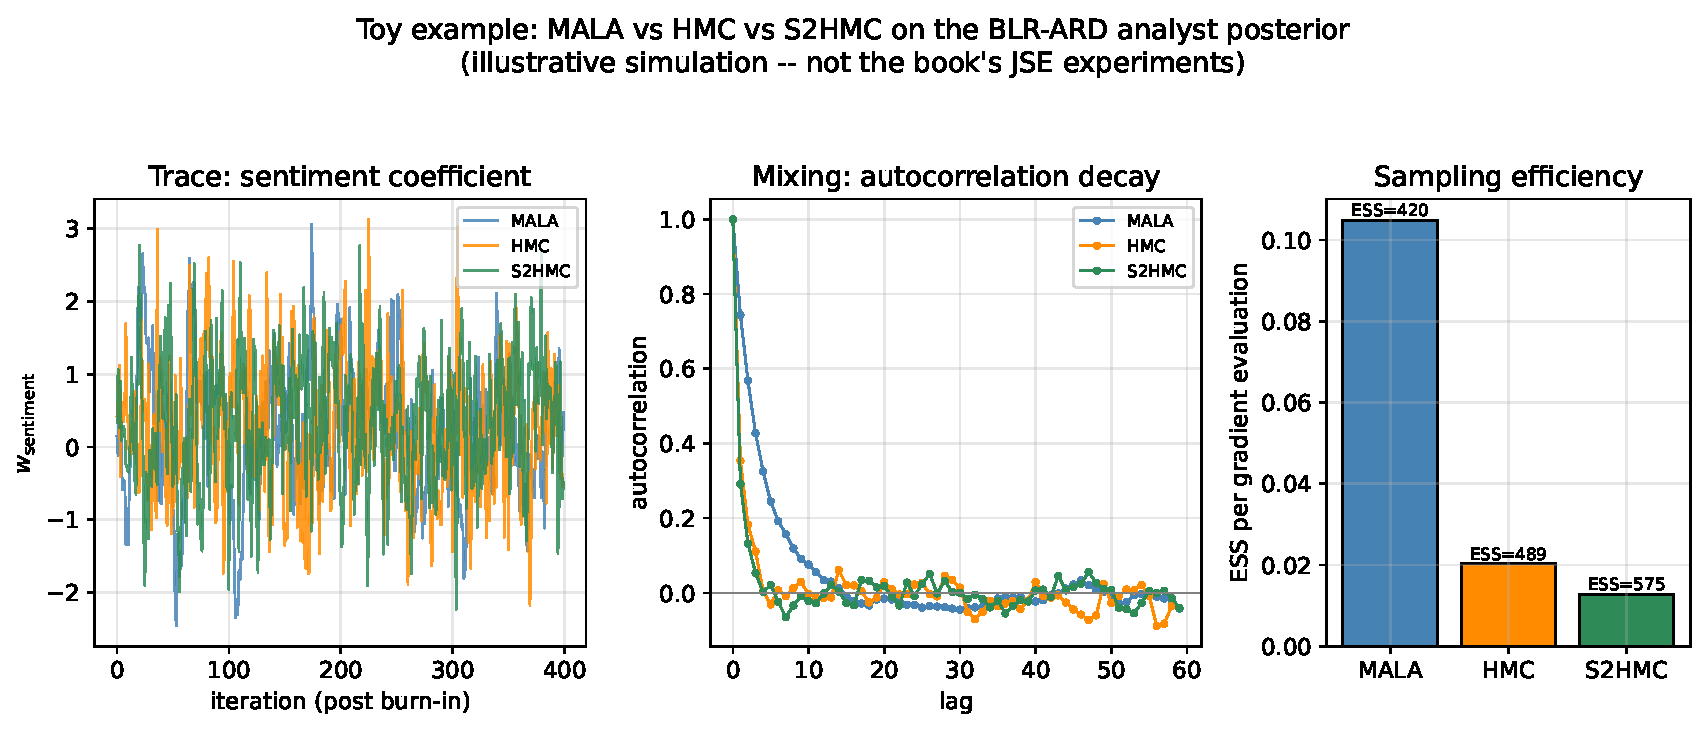
\includegraphics[width=0.95\linewidth]{fig_toy_mcmc_compare.pdf}
  \end{center}
  {\footnotesize \textbf{Left:} trace of the sentiment coefficient.
  \textbf{Middle:} autocorrelation decays fastest for HMC/S2HMC.
  \textbf{Right:} raw ESS grows MALA $<$ HMC $<$ S2HMC (matching the book's
  qualitative finding for the real JSE data, Sect.~13.5), but S2HMC's extra
  gradient evaluations per iteration (shadow maps) mean it needs the most
  compute per effective sample -- our grad-eval count is a cruder proxy than
  the book's wall-clock timings, but the direction of the effect agrees.}
\end{frame}

\begin{frame}{Toy Comparison: Predicted Bidirectional Accuracy}
  \begin{block}{Intuition}
    Fitting the toy BLR-ARD model via MALA (post burn-in posterior mean of
    $\w$) lets us predict $\hat p_i = \Ex[\sig(\w^\top x_i)\mid \Data]$ for
    each fictional report.
  \end{block}
  \begin{center}
    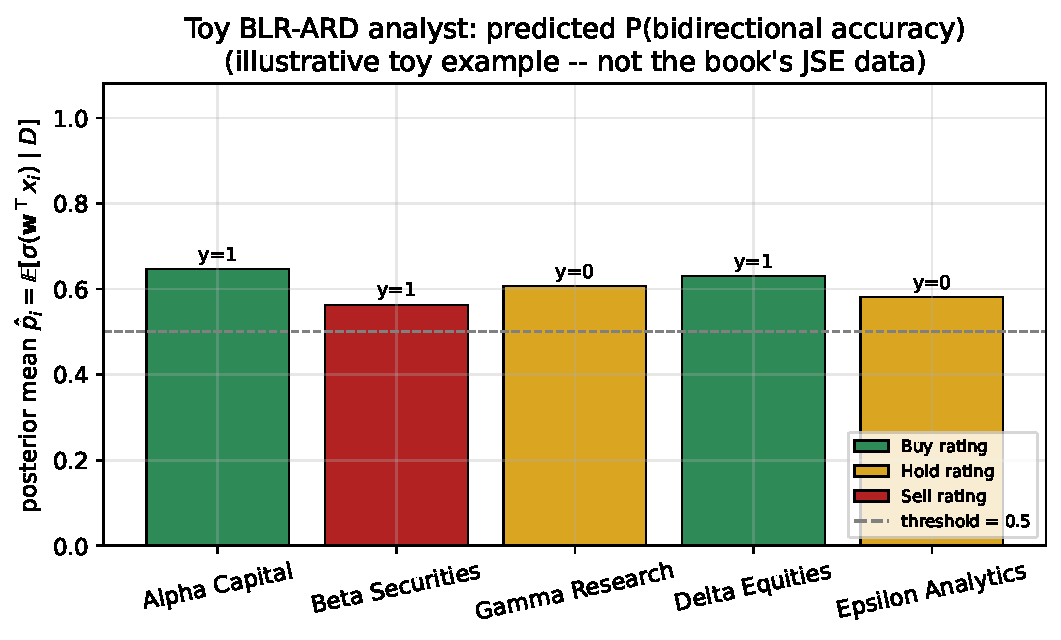
\includegraphics[width=0.72\linewidth]{fig_toy_analyst_predictions.pdf}
  \end{center}
  {\footnotesize Strong-conviction Buy/Sell calls (Alpha, Beta, Delta) are
  predicted correct with high probability; the wishy-washy "Hold" calls sit
  near the $0.5$ decision boundary -- Gamma Research lands \emph{exactly} at
  $0.5$, a nice illustration of the posterior being genuinely unsure about
  low-conviction reports, and Epsilon Analytics is a borderline miss,
  reminding us that even a Bayesian model is not immune to misclassifying
  edge cases with only 5 training points.}
\end{frame}

%%=============================================================================
\section{13.4 Numerical Experiments}
%%=============================================================================

\begin{frame}{13.4.1 \; Data Description}
  \begin{block}{The Real JSE Dataset}
    Sell-side analyst reports on \textbf{FTSE/JSE All Share Index}
    companies, sourced from \textbf{Bloomberg}, \textbf{11 Nov 2005 -- 29 Jun
    2018}: \textbf{29{,}935 reports} in total. Target: \textbf{bidirectional
    accuracy} of the initial-to-realised-closing-price move over a
    \textbf{12-month} horizon. Class balance: \textbf{56\% positive / 44\%
    negative}.
  \end{block}
  \begin{columns}
    \column{0.5\textwidth}
      {\footnotesize
      \textbf{14 features per report:}
      \begin{enumerate}
        \item Firm (report issuer)
        \item Target Price
        \item Rating (1=Strong Sell,\ldots,5=Strong Buy)
        \item $P_0$ (initial price)
        \item $\mathrm{TP}/P_0$
      \end{enumerate}}
    \column{0.5\textwidth}
      {\footnotesize
      \begin{enumerate}
        \setcounter{enumi}{5}
        \item 20-day rolling volatility
        \item Top40 cross-sectional volatility (CSV)
        \item RelVol (rolling vol / Top40 CSV)
        \item DAS (directional accuracy score)
        \item MES, MAS (met-end / met-any score)
        \item PAS (point accuracy score), PTM (price-target momentum), AC (analyst coverage)
      \end{enumerate}}
  \end{columns}
\end{frame}

\begin{frame}{13.4.2 \; Experiment Description}
  \begin{block}{Setup}
    \begin{itemize}
      \item \textbf{80/20 train-test split}; features min-max scaled.
      \item \textbf{2{,}500 posterior samples} generated per run, of which
            \textbf{1{,}000 are burn-in} (used for step-size tuning).
      \item Step size tuned by \textbf{primal-dual averaging} (Hoffman \&
            Gelman, 2014) targeting \textbf{60\% acceptance for MALA},
            \textbf{80\% for HMC and S2HMC}; trajectory length of HMC/S2HMC
            \textbf{fixed at $L=15$}.
    \end{itemize}
  \end{block}
  \begin{block}{Table 13.1: The Four Experiments}
    \begin{center}
    \begin{tabular}{clc}
      \toprule
      Experiment & Description & \# Observations\\
      \midrule
      1 & Full dataset             & 29{,}935\\
      2 & Resource stocks only     & 10{,}522\\
      3 & Financial stocks only    & 7{,}193\\
      4 & Industrial stocks only   & 12{,}220\\
      \bottomrule
    \end{tabular}
    \end{center}
  \end{block}
\end{frame}

\begin{frame}{13.4.3 \; Performance Metrics}
  \begin{block}{Sampler Diagnostics}
    \begin{itemize}
      \item \textbf{Trace plots} of the (un-normalised) target posterior.
      \item \textbf{Multivariate effective sample size (ESS)} (Vats et al.,
            2019) -- and ESS \textbf{normalised by execution time}, since a
            method that costs 10$\times$ more per sample needs 10$\times$
            the raw ESS just to break even.
    \end{itemize}
  \end{block}
  \begin{block}{Predictive Metric}
    \[
      \text{ROC: true positive rate vs.\ false positive rate}; \qquad
      \text{AUC = area under the ROC}
    \]
    AUC is preferred here because the relative cost of false positives vs.\
    false negatives is \emph{unknown} for the bidirectional-accuracy task --
    exactly the situation where AUC is the natural summary metric.
  \end{block}
\end{frame}

%%=============================================================================
\section{13.5 Results and Discussion}
%%=============================================================================

\begin{frame}{13.5 \; Predictive Performance (Table 13.2)}
  \begin{block}{AUC on Unseen Data (bold = best per experiment)}
    \begin{center}
    \begin{tabular}{lcccc}
      \toprule
      Algorithm & Exp.\ 1 & Exp.\ 2 & Exp.\ 3 & Exp.\ 4\\
      \midrule
      MALA  & 0.6181 & 0.6325 & 0.6154 & \textbf{0.6698}\\
      HMC   & \textbf{0.6182} & \textbf{0.6327} & 0.6158 & 0.6686\\
      S2HMC & \textbf{0.6182} & 0.6324 & \textbf{0.6164} & 0.6687\\
      \bottomrule
    \end{tabular}
    \end{center}
  \end{block}
  \begin{itemize}
    \item AUCs are \textbf{very close across all three samplers} within each
          experiment -- all three converge to essentially the same posterior
          predictive distribution, as they should.
    \item \textbf{Industrial stocks (Exp.\ 4)} give the highest AUC
          ($\approx 0.67$); \textbf{financial stocks (Exp.\ 3)} give the
          lowest ($\approx 0.615$-$0.616$), \emph{worse than the full
          dataset} -- financials are harder to call directionally.
    \item \textbf{Resource stocks (Exp.\ 2)} also outperform the full-dataset
          baseline.
  \end{itemize}
\end{frame}

\begin{frame}{13.5 \; Sampling Performance: ESS Across Methods}
  \begin{block}{Qualitative Findings (Figs.~13.1-13.3)}
    \begin{itemize}
      \item \textbf{MALA and HMC} give \textbf{similar} raw ESS, but with
            \textbf{wide confidence bands} across the four experiments.
      \item \textbf{S2HMC} gives \textbf{narrower confidence bands} -- a
            direct consequence of the shadow Hamiltonian being better
            conserved by the pre-processed leapfrog integrator.
      \item On a \textbf{time-normalised} basis, \textbf{S2HMC's ESS/time is
            much lower} than MALA's or HMC's, because its extra
            pre-/post-processing steps make each iteration far more
            expensive -- it buys better mixing \emph{per sample}, not
            \emph{per second}.
    \end{itemize}
  \end{block}
  \begin{block}{Diagnostics}
    All three methods show \textbf{flat negative-log-likelihood trace
    plots} after burn-in across all four experiments -- a visual confirmation
    of convergence for every sampler/experiment combination.
  \end{block}
\end{frame}

\begin{frame}{13.5 \; Which Features Matter? (Tables 13.3-13.5)}
  \begin{block}{Broad Agreement Across Samplers}
    The three MCMC methods broadly \textbf{agree} on which features matter
    most per sector, even though their numeric importance rankings are not
    identical:
  \end{block}
  \begin{itemize}
    \item \textbf{Full JSE universe (Exp.\ 1):} \emph{relative volatility}
          (RelVol) and \emph{initial price} ($P_0$) are the most consistently
          important features.
    \item \textbf{Resource stocks (Exp.\ 2):} \emph{20-day rolling
          volatility} and \emph{target price} dominate.
    \item \textbf{Financial stocks (Exp.\ 3):} \emph{analyst coverage},
          \emph{initial price}, and \emph{target price} matter most.
    \item \textbf{Industrial stocks (Exp.\ 4):} \emph{target price},
          \emph{initial price}, \emph{analyst coverage}, and \emph{Top40
          cross-sectional volatility} are essential.
  \end{itemize}
  \begin{alertblock}{Takeaway for Stakeholders}
    \textbf{Volatility context and price-level features consistently beat
    the raw rating/sentiment fields} -- and which exact feature dominates
    \textbf{differs by sector}, showing that a one-size-fits-all feature set
    is suboptimal for institutional investors screening sell-side reports.
  \end{alertblock}
\end{frame}

%%=============================================================================
\section{13.6 Conclusion}
%%=============================================================================

\begin{frame}[allowframebreaks]{13.6 \; Conclusion}

\begin{block}{What This Chapter Did}
Introduced a \textbf{Bayesian investment analyst}: a \textbf{Bayesian
logistic regression with ARD prior} (BLR-ARD) that predicts the
\textbf{bidirectional accuracy} of sell-side analyst reports on the JSE,
trained with \textbf{MALA, HMC, and S2HMC} and compared across all three.
\end{block}

\begin{block}{Key Results}
\begin{itemize}
  \item All three MCMC methods give \textbf{similar predictive AUC} --
        the choice of sampler does not change \emph{what} the model learns,
        only \emph{how efficiently} it explores the posterior.
  \item The model \textbf{outperforms on industrial and resource stocks},
        with \textbf{financial stocks} the hardest sector to call.
  \item The BLR-ARD's automatic feature ranking is a genuine practical
        payoff: institutional investors get a \emph{sector-specific} guide
        to which report features to focus on when challenging fund
        managers' strategies.
\end{itemize}
\end{block}

\framebreak

\begin{block}{Sampler Trade-off, Restated}
\begin{itemize}
  \item \textbf{MALA}: cheapest per iteration, most auto-correlated.
  \item \textbf{HMC}: similar ESS to MALA but with a longer, gradient-guided
        trajectory ($L=15$); good general-purpose middle ground.
  \item \textbf{S2HMC}: best raw ESS and narrowest ESS confidence bands, but
        the highest per-iteration cost -- worst ESS/time of the three here.
\end{itemize}
There is \textbf{no free lunch}: better mixing per sample does not
automatically mean better mixing per unit of wall-clock time.
\end{block}

\begin{alertblock}{Future Directions (as stated in the book)}
\begin{itemize}
  \item Replace BLR-ARD with more expressive models, e.g.\ \textbf{Bayesian
        neural networks}.
  \item Train per-sector "expert" models and \textbf{aggregate} them, e.g.\
        via \textbf{distributed Gaussian process} models (product-of-experts).
\end{itemize}
The next chapter concludes the book with a broader discussion of future
research directions in Bayesian quantitative finance.
\end{alertblock}

\end{frame}

\end{document}
